\newcommand{\comps}{\Lambda}
\newcommand{\pn}{\mathcal{N}}
%%%%%%%%%%%%%%%%%%%%%%%%%%%%%%%%%%%%%%%%%%%%%%%%%%%%%%%%%%%%%%%%%%%%%%%%%%%%%%
  \headerbox{Synthesis via Petri Net}{name=contribution,column=3,row=0}{
%%%%%%%%%%%%%%%%%%%%%%%%%%%%%%%%%%%%%%%%%%%%%%%%%%%%%%%%%%%%%%%%%%%%%%%%%%%%%%

\begin{multicols}{2}
Places:
 \begin{compactitem}
\item Types
 \end{compactitem}

Transitions:
\begin{compactitem}
\item API methods %(components)
\end{compactitem}
 \end{multicols}

   \noindent{\centering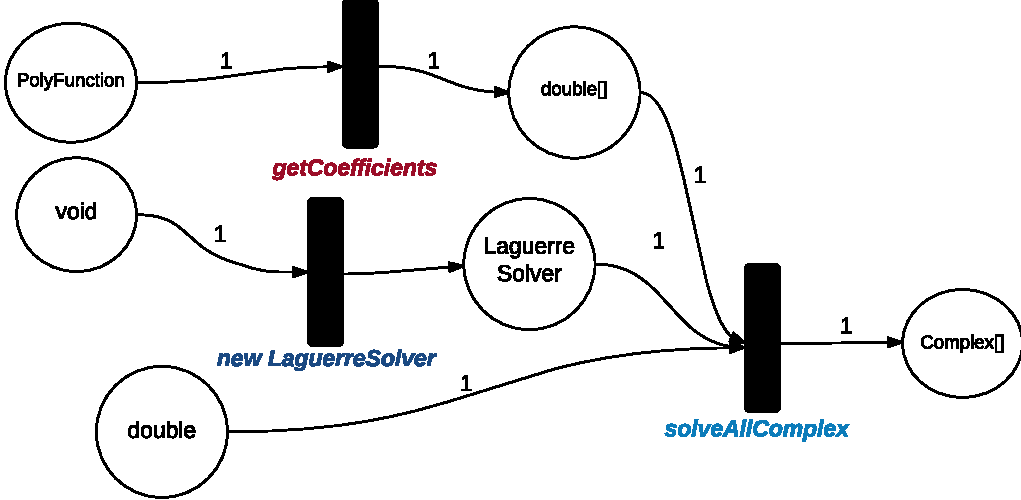
\includegraphics[scale=0.45]{images/net.pdf}\\}
 %{\sc SyPet} first constructs a Petri net $\pn$ using \emph{signatures} of components in $\comps$.
 %where the places of $\pn$ correspond to types and transitions correspond to components. Then it performs reachability analysis to find $\pn$'s accepting runs. For instance, an accepting run $r$ is  \code{new LaguerreSolver}, \code{getCoefficients}, \code{solveAllComplex}. 

 A reachable path in the Petri net corresponds to a program sketch. For example:
 \begin{compactitem}
 \item \code{new LaguerreSolver}
 \item \code{getCoefficients}
 \item \code{solveAllComplex}
 \end{compactitem}

   \vspace{0.3em}
  }


